\documentclass{article}
\usepackage[utf8]{inputenc}
\usepackage{subfig}
\usepackage{amsmath}

\usepackage{graphicx}
\usepackage[legalpaper, portrait, margin=0.5cm]{geometry}
\renewcommand{\thesubfigure}{\roman{subfigure}}

\thispagestyle{empty}
\begin{document}

\begin{figure}[h]
        \centering

        \subfloat[$N$=1]{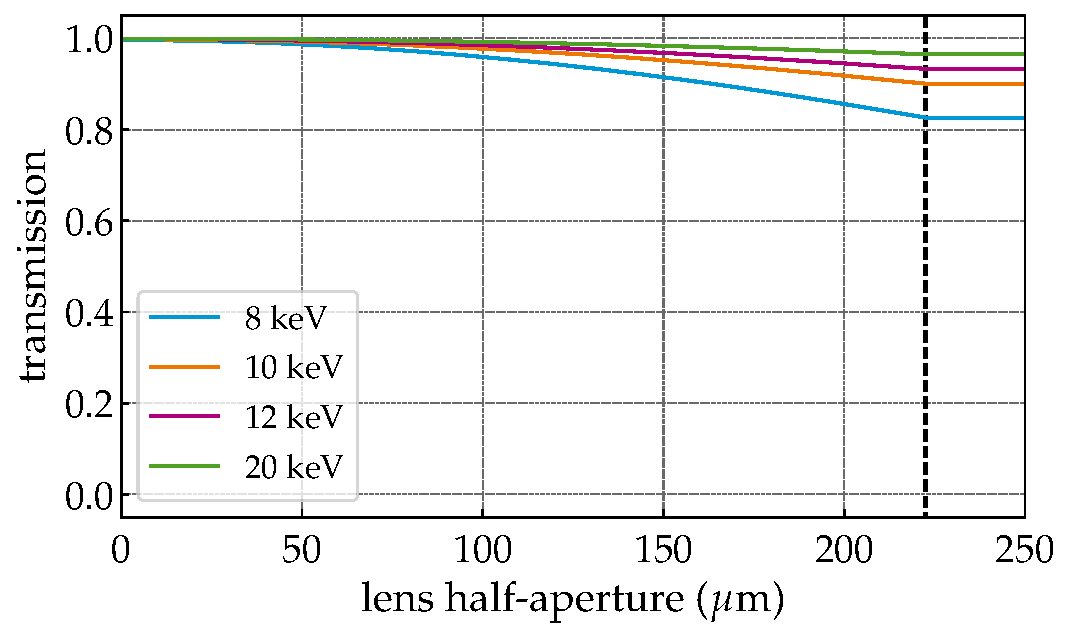
\includegraphics[height=3.5cm]{figures/ch03/Aeff_1.pdf}}\hspace{0.2cm}
        \subfloat[$N$=10]{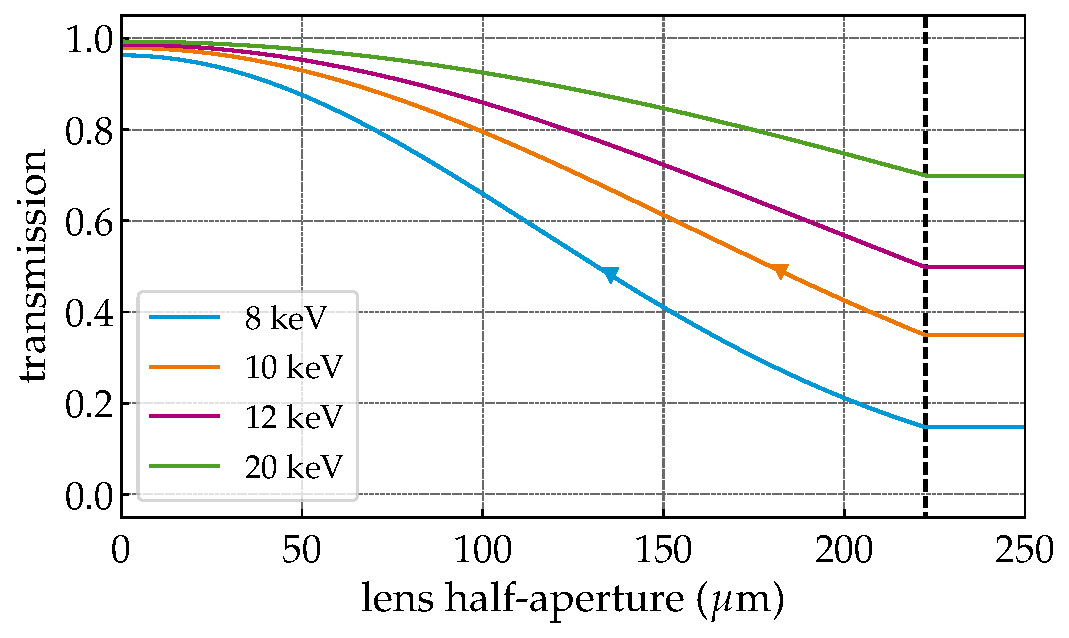
\includegraphics[height=3.5cm]{figures/ch03/Aeff_10.pdf}}\hspace{0.2cm}
        \subfloat[$N$=20]{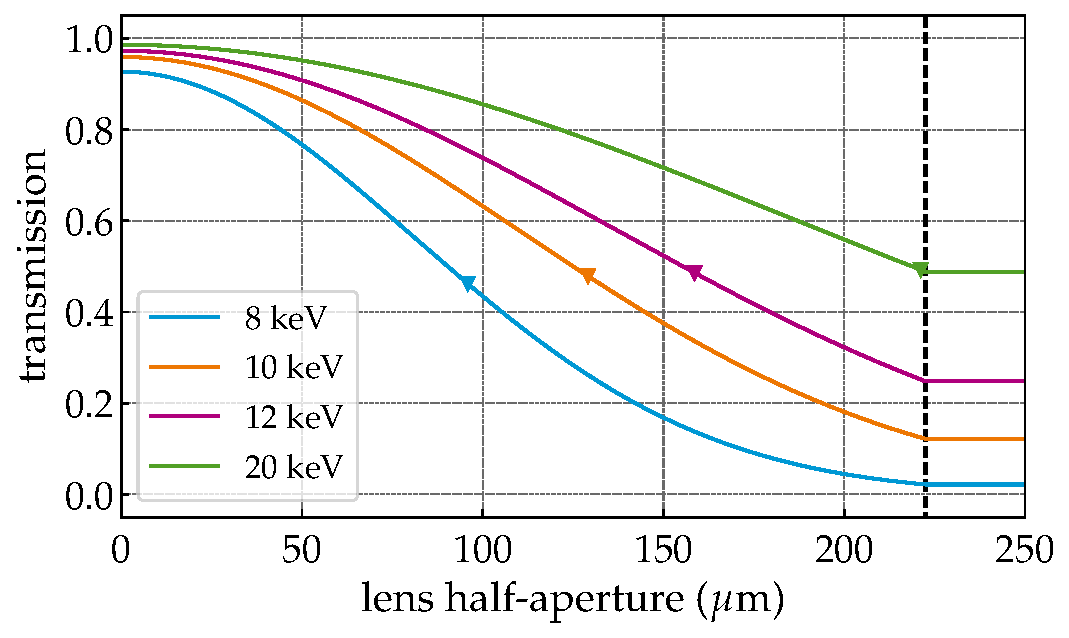
\includegraphics[height=3.5cm]{figures/ch03/Aeff_20.pdf}}\\\setcounter{subfigure}{0}
        \caption*{(a) intensity transmission}
        \subfloat[$N$=1]{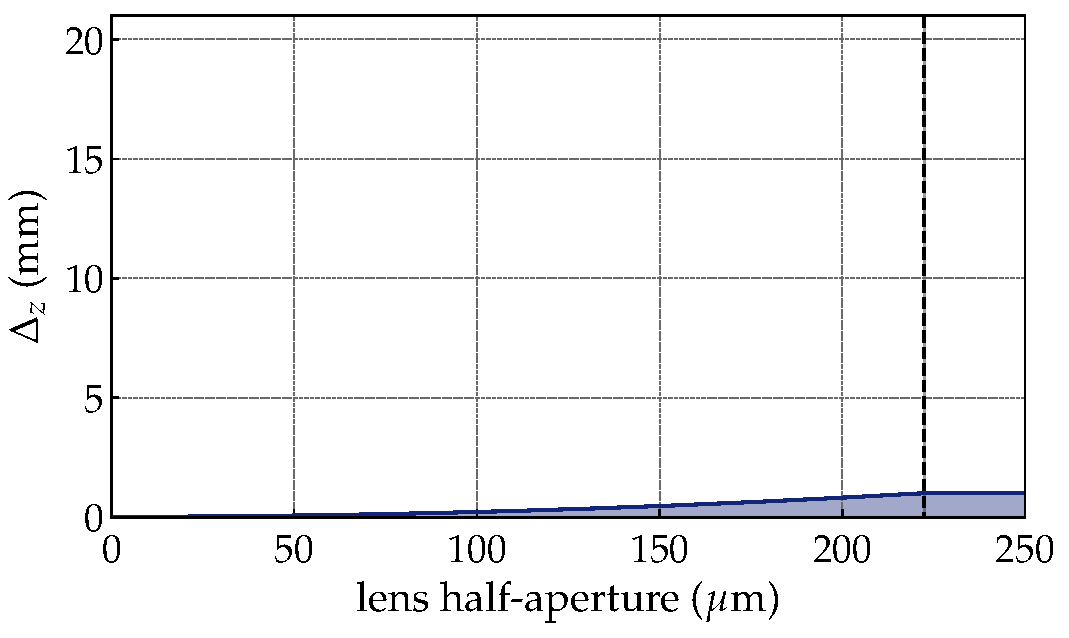
\includegraphics[height=3.5cm]{figures/ch03/Acc_1.pdf}}\hspace{0.2cm}
        \subfloat[$N$=10]{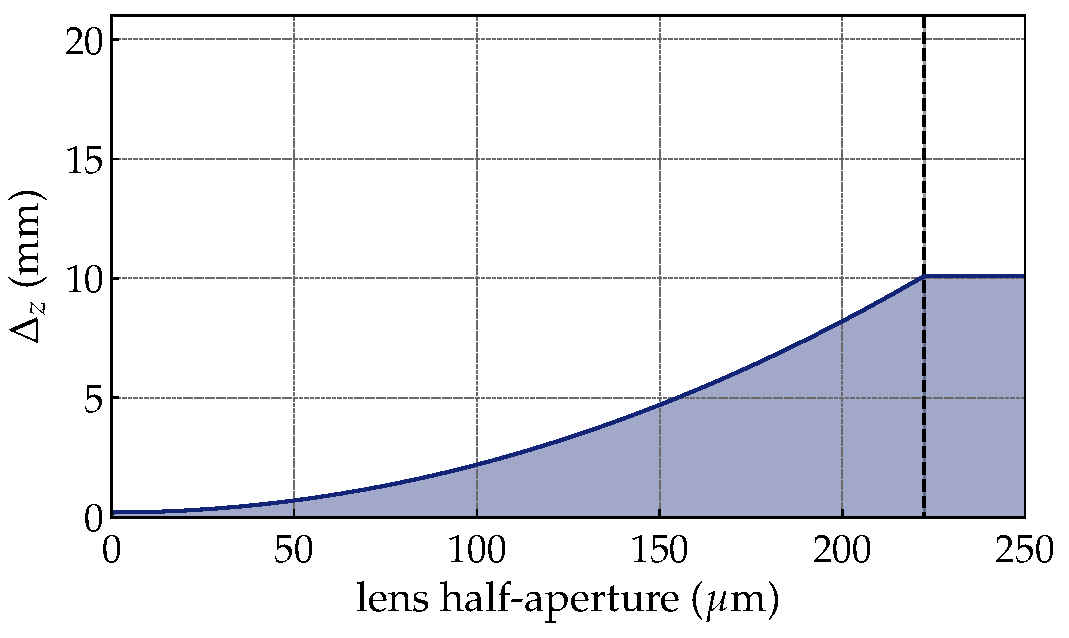
\includegraphics[height=3.5cm]{figures/ch03/Acc_10.pdf}}\hspace{0.2cm}
        \subfloat[$N$=20]{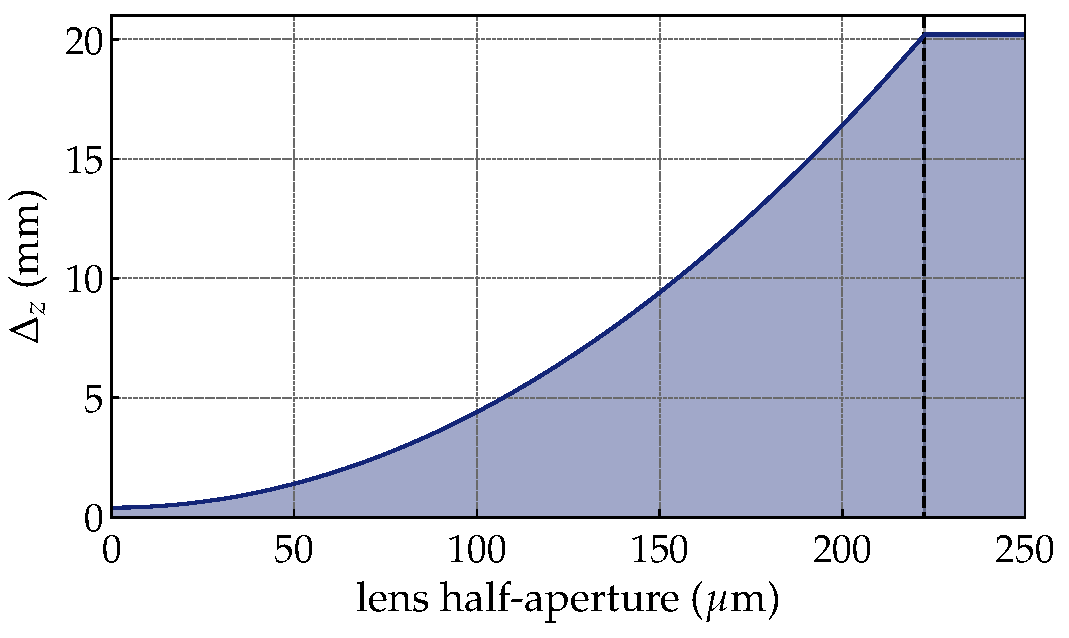
\includegraphics[height=3.5cm]{figures/ch03/Acc_20.pdf}}
        \caption*{(b) accumulated thickness $\Delta_z$}

        
        
\end{figure}
\end{document}


\end{document}